\documentclass{article}
\title{Nechyba Ch.16 一般均衡}
\author{Dawei Wang}
\date{\today}
\usepackage{ctex}
\usepackage{amsmath}
\usepackage{amssymb}
\usepackage{graphicx} %插入图片的宏包
\usepackage{float} %设置图片浮动位置的宏包
\usepackage{subfigure} %插入多图时用子图显示的宏包
\begin{document}
	\maketitle
一般均衡模型(general equilibrium models)把整个经济视作关联市场的一个封闭的系统,明确而具体地考虑局部均衡分析的假设里忽略的影响。

“福利经济学第二定理”是一个被称为“核”的资源配置稳定性的概念,以及这个“核”事实上收敛到通过分散的市场势力所产生的结果。

\section{一般均衡的图示阐述}

在市场经济中发生了三种基本的经济活动:生产、交换、以及源于这些活动的消费。

\subsection{纯交换经济}

纯交换经济(pure exchange economy)被定义为一个没有生产,并且消费者被赋予不同商品束的经济。

更正式地,将小经济定义为:(1)经济中的个体;(2)我们对商品的偏好;(3)在经济中我们所拥有的商品的禀赋。

\begin{figure}[H] %H为当前位置,!htb为忽略美学标准,htbp为浮动图形
	\centering %图片居中^{}
	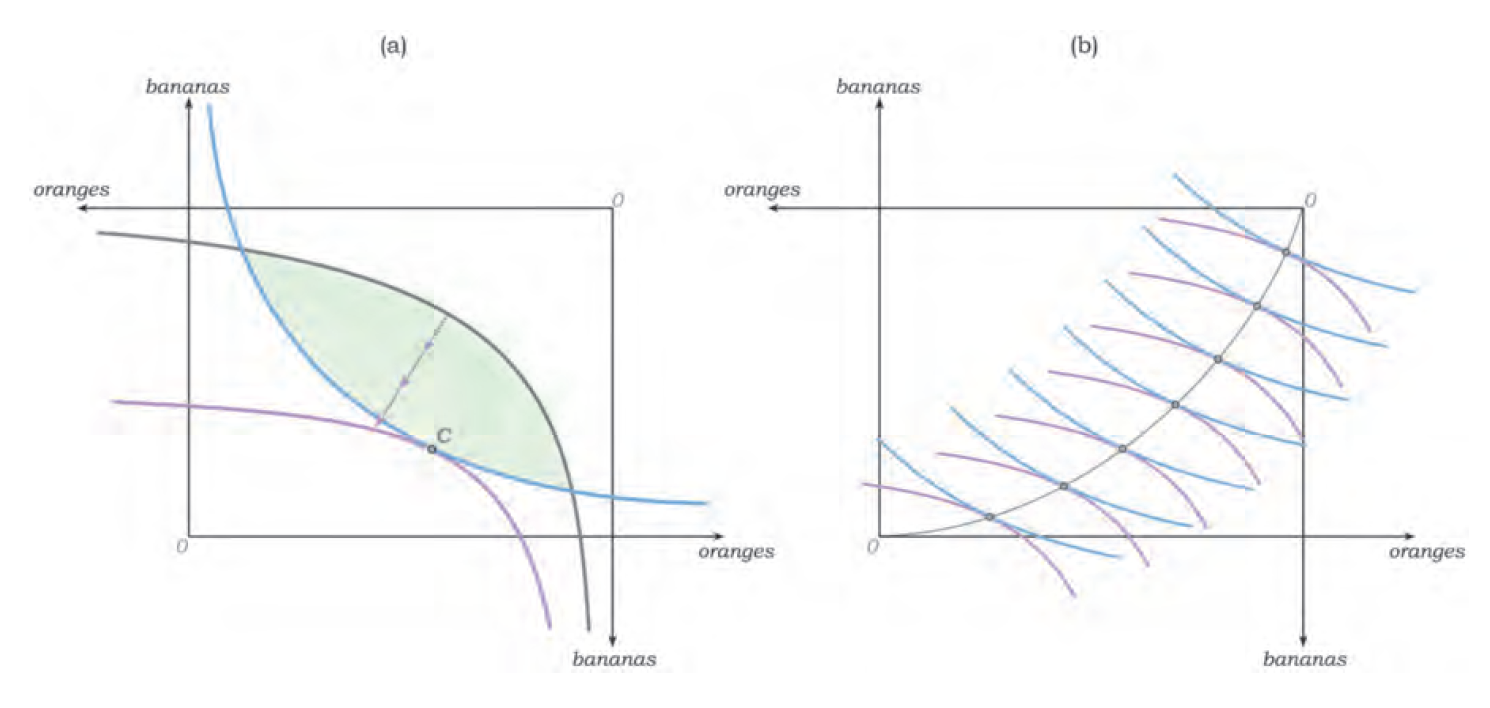
\includegraphics[width=1\textwidth]{16_1} %插入图片,[]中设置图片大小,{}中是图片文件名
	\caption{The Contract Curve: Pareto Efficient Allocations in the Edgeworth Box} %最终文档中希望显示的图片标题
	\label{Fig.main2} %用于文内引用的标签
\end{figure}

不管经济中的初始禀赋落在什么地方,个体将会找到导致经济禀赋的有效配置的交易(或“契约”),经济禀赋的Pareto有效配置的全集称为契约曲线(contract curve)。

交易双方将(1)在到达契约曲线之上的有效配置之前一直交易;(2)交易双方任何人都不会比在各自的禀赋点(E)更差是合理的。

\begin{figure}[H] %H为当前位置,!htb为忽略美学标准,htbp为浮动图形
	\centering %图片居中^{}
	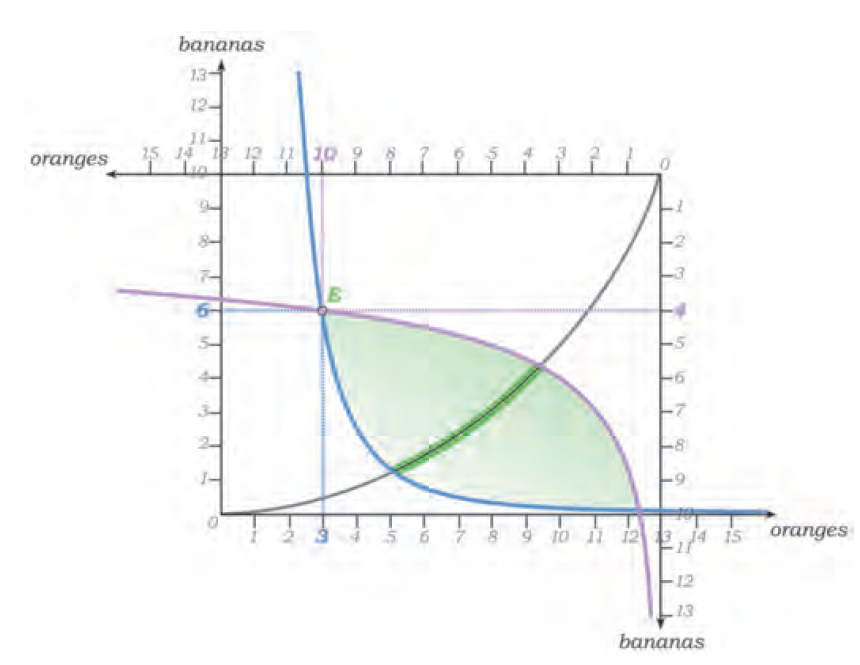
\includegraphics[width=1\textwidth]{16_2} %插入图片,[]中设置图片大小,{}中是图片文件名
	\caption{The Contract Curve: Pareto Efficient Allocations in the Edgeworth Box} %最终文档中希望显示的图片标题
	\label{Fig.main3} %用于文内引用的标签
\end{figure}

画出交易双方仅消费禀赋所能获得的无差异曲线、表示二者都能变得更好的配置集的阴影区域,以及表示无差异曲线相切的有效配置的线。交易双方将(1)耗尽所有交易的收益;(2)仅同意提高交易双方福利的交易的预测意味着交易双方能认同的可能配置将位于契约曲线的粗体线段部分。

契约曲线上这个粗体线段通常被称为二人交换经济的核。一个配置位于核当中当且仅当经济中不存在个体的子集通过相互交易可以使得他们变得更好。在只有两个个体的交换经济的例子中,这意味着,为使禀赋的配置位于核中,这两个个体无法相处一种方式使得双方都变得更好。

当经济由多于两个个体组成时,核通常是契约曲线粗体部分的一个子集。

\subsubsection{Edgeworth 图中的竞争性均衡}

唯一使供给等于需求的方式是,在所报价格下,交易一方愿意放弃的某商品数量与另一方愿意买的恰好一样多并且另一方愿意放弃的另一商品的数量恰好等于该方愿意购买的数量。

\begin{figure}[H] %H为当前位置,!htb为忽略美学标准,htbp为浮动图形
	\centering %图片居中^{}
	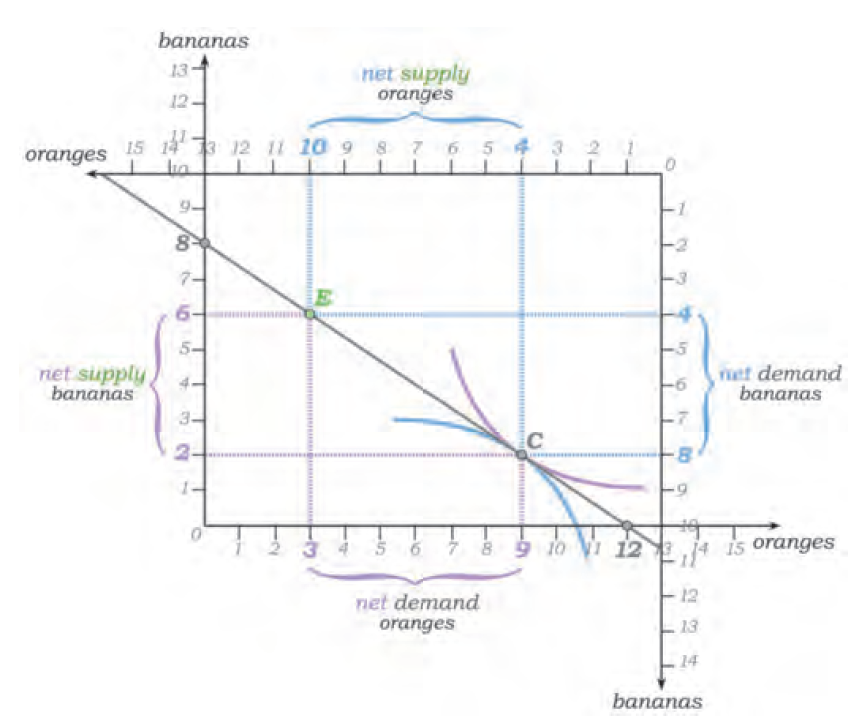
\includegraphics[width=1\textwidth]{16_3} %插入图片,[]中设置图片大小,{}中是图片文件名
	\caption{Competitive Equilibrium Prices: Supply Equals Demand} %最终文档中希望显示的图片标题
	\label{Fig.main4} %用于文内引用的标签
\end{figure}

为什么在一个两人经济中的个体会是价格接收者呢?在这样一个环境下,假定两个个体通过讨价还价而不是假定某个固定的价格来找到他们达到有效结果的方式是更加合理的。但是这里我们把自己限制在两人交换经济中的唯一原因是它允许我们图示一些基本的直觉并推导一些本质的结果。结果显示,相同的直觉对更大的经济体也奏效,在该经济体中有很多个体,由于每个相对于经济体很小,使得我们可以合理地假设他们把价格当成既定地。

\subsection{福利经济学基本定理与其他结果}

福利经济学第二定理:只要政府能以一次性转移的方式重新分配禀赋,任何有效的配置实际上都是市场均衡。

已经被证明的是,随着经济体变大,经济的核收缩到仅为市场均衡结果的集合,这是我们称之为核收敛的结果。

由于可以合理地预期个体利用他们讨价还价的技能,相互之间进行交易直到个体讨价还价的能力被稀释时竞争性均衡结果实际上是我们应该预期会产生的唯一结果。

只要最初的禀赋被适当的重新分配,任何帕累托有效的配置都能产生于竞争性均衡。从而福利经济学第一定理说竞争性均衡是帕累托有效的,而福利经济学第二定理则说任何有效的配置可以是一个竞争性均衡,只要政府能重新分配禀赋,并且在这一过程中经济不收缩。

如果D要成为一个均衡配置,则一定时我们能在Edgeworth盒状图中画一个预算约束经过D并且在点D两条无差异曲线的斜率完全相同。 但是,由于预算线总是通过禀赋点,那么该直线成为预算约束的唯一方式是我们的禀赋点位于该直线上。福利经济学第二定理说的是只要初始禀赋被合理地重新分配,任何有效的配置都能成为均衡配置。

该定理的隐含假设是我们能无成本地进行再分配,以及我们可以再分配而不收缩经济的大小。换言之,福利经济学第二定理假设“总量转移再分配”——通过一次性总量税收和补贴再分配——是可能的。换言之,通过现实世界(扭曲的)税收和补贴获得的再分配收缩了经济。从而,由于现实世界再分配会导致无效性,从而不太可能像福利经济学第二定理所预想的那样“适当地再分配”。由此,如果经济中的禀赋被不公平地分配了,导致了有效但是不公平的结果,那么公平和有效之间的权衡取舍便产生了,再分配导致了非有效性但是潜在地有更多公平。

假设个体将会继续交易直到没有进一步的互利交易是合理的,这将意味着他们最终将位于核中的某个经济禀赋的配置处。

随着一个交换经济变得“更大”,核配置的集合收缩;当经济的规模变得非常大时,核收缩到恰好是竞争性均衡配置的集合。从而,如果我们要通过简单地找到所有位于经济中“核”的配置来预测在一个大的交换经济中谁得到什么,这将是与找到所有竞争性市场价格支撑的配置的集合完全相同的练习。换言之,在大的经济中,只有稳定的配置才能作为竞争性均衡产生,并且不能作为竞争性均衡产生的配置没有这种稳定性。

在较大的经济体中,来自其他参与人的竞争降低了个体的讨价还价能力。

\subsection{Robinson Crusoe生产经济}

若我独自在一个岛上,岛上生长的唯一食物就是香蕉。可以把我想象成一个生产者和一个消费者:我是一个用劳动生产香蕉的生产者,并且我是一个吃放弃休闲的消费者。



\begin{figure}[H] %H为当前位置,!htb为忽略美学标准,htbp为浮动图形
	\centering %图片居中^{}
	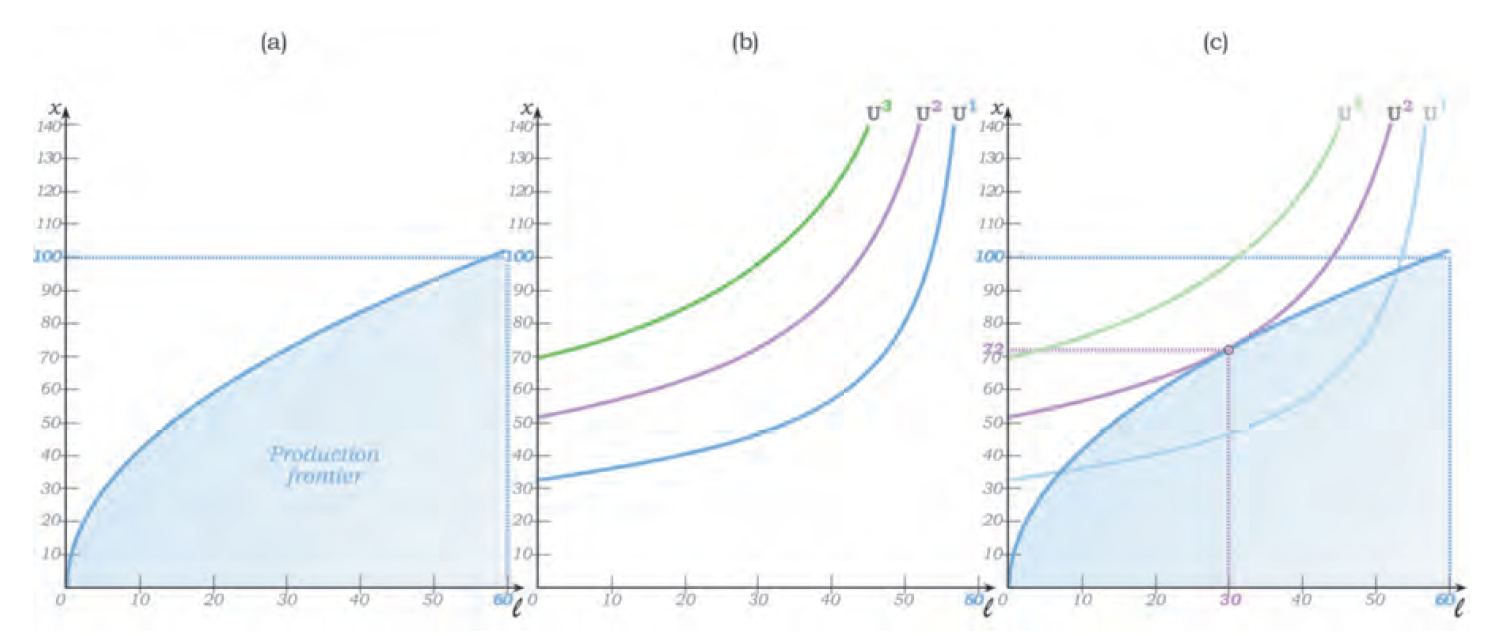
\includegraphics[width=1\textwidth]{16_4} %插入图片,[]中设置图片大小,{}中是图片文件名
	\caption{Robinson Crusoe Choosing His Optimal Bundle} %最终文档中希望显示的图片标题
	\label{Fig.main5} %用于文内引用的标签
\end{figure}

假设我人格分裂,我的一部分仅作为一个利润最大化的生产者,而我的另一部分仅作为一个效用最大化的消费者。进一步假定我的两部分都表现为价格接受者,把劳动的价格w和香蕉的价格p当成既定的。

\begin{figure}[H] %H为当前位置,!htb为忽略美学标准,htbp为浮动图形
	\centering %图片居中^{}
	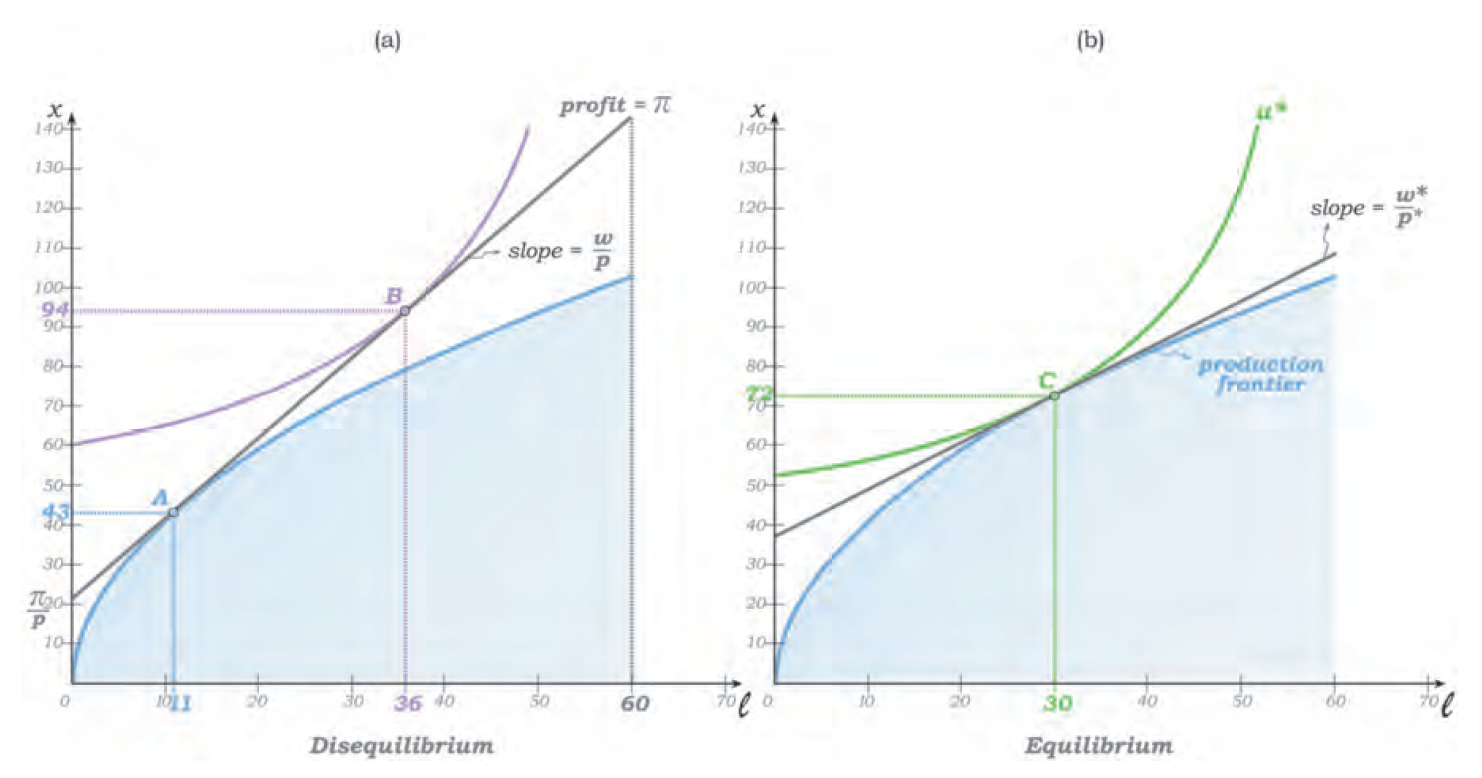
\includegraphics[width=1\textwidth]{16_5} %插入图片,[]中设置图片大小,{}中是图片文件名
	\caption{} %最终文档中希望显示的图片标题
	\label{Fig.main6} %用于文内引用的标签
\end{figure}


为了使这个经济处于均衡,p和w必须改变使得生产者的最优生产计划与消费者的最优消费计划一致。

\hspace*{\fill}

福利经济学第一和第二定理

福利经济学第一定理是指定条件使得竞争性均衡是Pareto有效的定理。在一个有着单一个体的经济中,Pareto有效仅意味着单一个体,正在最优化他的行为。于是我们找到了仍包含一个可行消费束的最高的无差异曲线。

福利经济学第二定理说的是经济中任何Pareto最优可以作为一个均衡被支持。福利经济学仅在生产选择集和偏好为凸时才能确保成立。

\subsection{一般均衡分析与政策}

税收和补贴会改变特定市场的价格。有时,这些变化以这样一种方式发生使得我们能孤立一个市场并卓有成效地分析,而不用考虑经济中的一般均衡,但是经常地,即使一个政策明确地仅改变了一个单一市场价格,紧随其后的个体决策也会使影响以重要的方式“外溢”到其他市场中。经济学家已经证明紧随政策变化的一般均衡效应通常比政策制定者心目中最前面的最初的局部均衡效应更重要。

\section{竞争性一般均衡}

\subsection{纯交换经济}

把交换经济定义为有着禀赋和偏好的消费者的集合。例如,假定经济包含N个消费者(记为n=1,n=2,...,M)。一个纯交换经济被完全定义为:
\[
(\{(e^n_1,e^n_2,\cdots,e^n_m)\}_n^N=1, \{u^n:\mathbb{R}^M\rightarrow\mathbb{R}^1\}^N_n=1)
\]

其中,$ (\{(e^n_1,e^n_2,\cdots,e^n_m)\}_n^N=1 $给出了个体n的M种商品中的禀赋,$ u^n:\mathbb{R}^M\rightarrow\mathbb{R}^1 $是个体n在M种商品上的效用函数。记号$ \{\}_n^N=1 $简单地表示出现在花括号中的是对经济中N个不同的消费者列出来的。$ e^n_m $读作“个体n的商品m的禀赋”。

只要我们对一种商品的配置没有超过总体上可以得到的,任何其他个体之间的商品的配置就是可行的。对任何商品m,我们定义经济的总体禀赋$ E_m $为简单把所有个体禀赋加总,即:

\[
E_m=e^1_m+e^2_m+\cdots+e^N_m
\]

定义一个交换经济中的可行配置集(set of feasible allocation)FA为

\begin{equation*}
	\begin{split}
	FA=\{\{(x_1^n,x_2^n\cdots,x_M^n)\}^N_{n=1}\in \mathbb{R}^{NM}_+|&x_m^1+x_m^2+\cdots+x_m^N=E_m,\\
	&\enspace for\enspace all\enspace n=1,2,\cdots,M\}
	\end{split}
\end{equation*}

\hspace*{\fill}

互利交易

我们称这种用在自己身上获得的效用水平为我们的保留效用。为了使交易是互利的,源于交易的经济禀赋的划分必须至少给予我们每个人我们的保留效用。令个体n的保留效用记为$ U^n $,我们简单地评价禀赋处的效用计算出适当的保留效用值;即

\[
U^n=u^n(e^n_1,e^n_2,\cdots,e^n_M)
\]

经济中对每个人都是互利的(经济的禀赋的)配置的集合(记为MB),为至少给予每个消费者ta的保留效用的可行配置集;即

\begin{equation*}
\begin{split}
FA=\{\{(x_1^n,x_2^n\cdots,x_M^n)\}^N_{n=1}\in FA|&u^n(x_m^1+x_m^2+\cdots+x_m^N)\ge U_n,\\
&\enspace for\enspace all\enspace n=1,2,\cdots,M\}
\end{split}
\end{equation*}

\hspace*{\fill}

契约曲线

并不是所有的互利交易一定导致Pareto有效配置,同样并不是所有有效的配置都位于互利交易的透镜状区域内。

定义集合:

\begin{equation*}
\begin{split}
FA=&\{\{(x_1^n,x_2^n\cdots,x_M^n)\}^N_{n=1}\in FA|there\enspace does\enspace not\enspace exist\{(y_1^n,y_2^n\cdots,y_M^n)\}^N_{n=1}\in FA\\
&where\enspace u^n(y_1^n,y_2^n\cdots,y_M^n)\ge u^n(x_1^n,x_2^n\cdots,x_M^n),\enspace for\enspace all\enspace n=1,2,\cdots,N\\
&and\enspace u^n(y_1^n,y_2^n\cdots,y_M^n)> u^n(x_1^n,x_2^n\cdots,x_M^n),\enspace for \enspace some\enspace n\}
\end{split}
\end{equation*}

\hspace*{\fill}

核

\[
Core=MB\cap PE
\]

更一般地,核被定义为配置的集合,在其中没有个体的“联合”使他们自己能做得更好
。

\hspace*{\fill}

\textbf{竞争性均衡}

\textbf{在均衡中,商品的市场价格必须使得供给等于需求。}消费者n变成商品m的净供给者,如果在市场价格下ta的需求小于ta的禀赋;消费者成为一个净需求者,如果ta的需求大于ta的禀赋。

\[
x^1_1(p_1,p_2,(p_1e^1_1+p_2e^1_2))+x^2_1(p_1,p_2,(p_1e^2_1+p_2e^2_2)-e^2_2)=e^1_1+e^2_1
\]
\[
x^1_2(p_1,p_2,(p_1e^1_1+p_2e^1_2))+x^2_2(p_1,p_2,(p_1e^2_1+p_2e^2_2)-e^2_2)=e^1_2+e^2_2
\]

\hspace*{\fill}

瓦尔拉斯定律

每个个体的预算束在最优处是紧的;即在最优处,一个消费者的无差异曲线与预算约束相切。在数学上,这对消费者n可以简单表述为$ p_1x_1^n+p_2x_2^n=p_1e_1^n+p_2e_2^n $;即消费者n的花费等于收入但是如果这对每个个体消费者都成立,那么它对整个经济体也成立:经济总体的预算约束是紧的。

在两人两商品经济中,经济的总体预算约束简单地变成:

\[
p_1(x^1_1+x^2_1)+p_2(x^1_2+x^2_2)=p_1(e^1_1+e^2_1)+p_2(e^1_2+e^2_2)
\]

更一般地,如果我们处理一个N人,M商品的交换经济,我们能写出M个不同的“需求等于供给”的方程,但是由于瓦尔拉斯定律。我们仅需要解$ (M-1) $个方程来求出M商品的相对价格,因为,如果在$ (M-1) $个市场中“需求等于供给成立”。那么其必然在最后一个市场中也成立。

\subsection{福利经济学基本定理与其他结果}

福利经济学第一定理

假定$ \{p_1,p_2,x^1_1,x^1_2,x^2_1,x^2_2\} $是由$ \{e^1_1,e^1_2,e^2_1,e^2_2,u^1,u^2\} $所定义的交换经济的竞争性均衡,其中$ u^1 $和$ u^2 $是表示两个人偏好的效用函数。

假定均衡配置$ (x^1_1,x^1_2,x^2_1,x^2_2) $不是有效的这将意味着存在经济中商品的另一个可行的配置使得没有人变得更差并且至少有一个人在这个配置下变得更好。我们称这个配置为$ (y^1_1,y^1_2,y^2_1,y^2_2) $。假定实际上两个人都在这个配置下变得更好。由于每个个体都在均衡价格$ (p_1,p_2) $处做到最好以达到均衡配置,则一定是$ (y^1_1,y^1_2) $对于个体1而言在均衡价格出负担不起并且$ (y^2_1,y^2_2) $在那些价格下对于个体2而言也负担不起,从而

\[
p_1y^1_1+p_2y^1_2>p_1x^1_1+p_2x^1_2\enspace and\enspace p_1y^2_1+p_2y^2_2>p_1x^2_1+p_2x^2_2
\]

把不等式两边相加意味着

\[
p_1(y^1_1+y^2_1)+p_2(y^1_2+y^2_2)>p_1(x^1_1+x^2_1)+p_2(x^1_2+x^2_2)
\]

该方程的右边为瓦尔拉斯定律,因而意味着

\[
p_1(y^1_1+y^2_1-e^1_1-e^2_1)+p_2(y^1_2+y^2_2-e^1_2-e^2_2)>0
\]

由于价格是正的,这意味着$ (y^1_1+y^2_1-e^1_1-e^2_1) $或$ (y^1_2+y^2_2-e^1_2-e^2_2) $两着至少一个大于零。即$ y^1_1+y^2_1>e^1_1+e^2_1\enspace and/or\enspace y^1_2+y^2_2>e^1_2+e^2_2 $,但这意味着配置$ (y^1_1,y^1_2,y^2_1,y^2_2) $是不可行的。

综上所述均衡配置$ (x^1_1,x^1_2,x^2_1,x^2_2) $一定是有效的。

\hspace*{\fill}

福利经济学第二定理

福利经济学第二定理指出存在一个经济禀赋的再分配使得契约曲线上的任何点在再分配后都可以被支撑为一个竞争性均衡。其证明要求假设偏好是凸的(福利经济学第一定理不要求这一点)。

福利经济学第一定理的强大之处在于它告诉我们存在条件使得竞争性均衡是有效的。而福利经济学第二定理不太强大,因为它假定我们能无成本地重新分配禀赋;即存在着我们在前面所称的不改变替代效应的“总量税”。它进一步假定我们有经济中个体的充分信息以使得我们能以正确的方式得到契约曲线上我们偏好的作为一个均衡产生的点。不过,福利经济学第二定理表明,只要禀赋的再分配是可能的,竞争性市场就可以用来得到一个比产生于经济禀赋的初始分配“更公平”的均衡结果。换言之,我们认为禀赋“不公平地”分配的事实并不意味着市场在再分配发生后不能起到有效性的作用。

\hspace*{\fill}

均衡与核

二人交换经济的竞争性均衡一定位于经济的“核”中。当经济中仅有两个消费者时,核就是Pareto有效配置中被每个个体共同偏好的禀赋的子集。福利经济学第一定理保证了竞争性均衡是Pareto有效的。进一步,个体最优化的逻辑意味着每个个体在均衡价格下愿意放弃ta的禀赋而转移到均衡配置。

当经济在每种类型有很多个体意义上扩张时,核收缩到竞争性均衡的集合。这被称为核收敛定理。由于核配置的集合是可行地产生于个体核群组的讨价还价的配置的集合,核收敛定理告诉我们当讨价还价的竞争由于大量的消费者而变得充分激烈时,每个人讨价还价的能力被充分地减少,这使得任何讨价还价过程地结果都变得与市场中竞争行为的结果相同。

\subsection{一个简单的Robinson Crusoe生产经济}

作为生产者,把香蕉价格p和工资w当成既定的,并求解利润最大化问题
\[
\max\limits_{x,l} px-wl\enspace s.t.\enspace x=f(l)
\]

解出要素需求函数和产出供给函数:

\[
l^D(w,p),x^S(w,p)
\]

作为消费者,给定休闲禀赋L,计算利润函数

\[
\pi(w,p)
\]

计算效用最大化问题

\[
\max\limits_{x,l}u(x,L-l)\enspace s.t.\enspace px=wl+\pi(w,p)
\]

解出劳动供给和香蕉需求:

\[
l^S(w,p),x^D(w,p)
\]

\hspace*{\fill}

Robinson Crusoe经济中的均衡

为了计算均衡,需要确保在劳动和产出市场中需求等于供给。然而由于瓦尔拉斯定律已经包含在解生产者问题和消费者问题的约束之中,故一个市场的均衡必然意味着另一个市场也处于均衡之中。

因此,令$ l^S=l^D $或$ x^S=x^D $即可求得均衡。

\section{结论}

当没有扭曲型力量发生时,竞争性均衡导致了稀缺资源的有效配置。

核与竞争性均衡配置的集合的关系表明,当经济变大时,个体的子群将永远不能对结果讨价还价,使得结果比他们在竞争性市场中得到的结果更好。因此,竞争均衡所要求的“价格接收者”的假设在经济变大时非常合理。

\end{document}